\documentclass[../Main.tex]{subfiles}

\begin{document}

\section{Resultados y Conclusiones}
Al aplicar el método anterior se puede realizar una predicción bastante acertada para varios de los circuitos eléctricos. A continuación se presentan algunos resultados.

\begin{center}
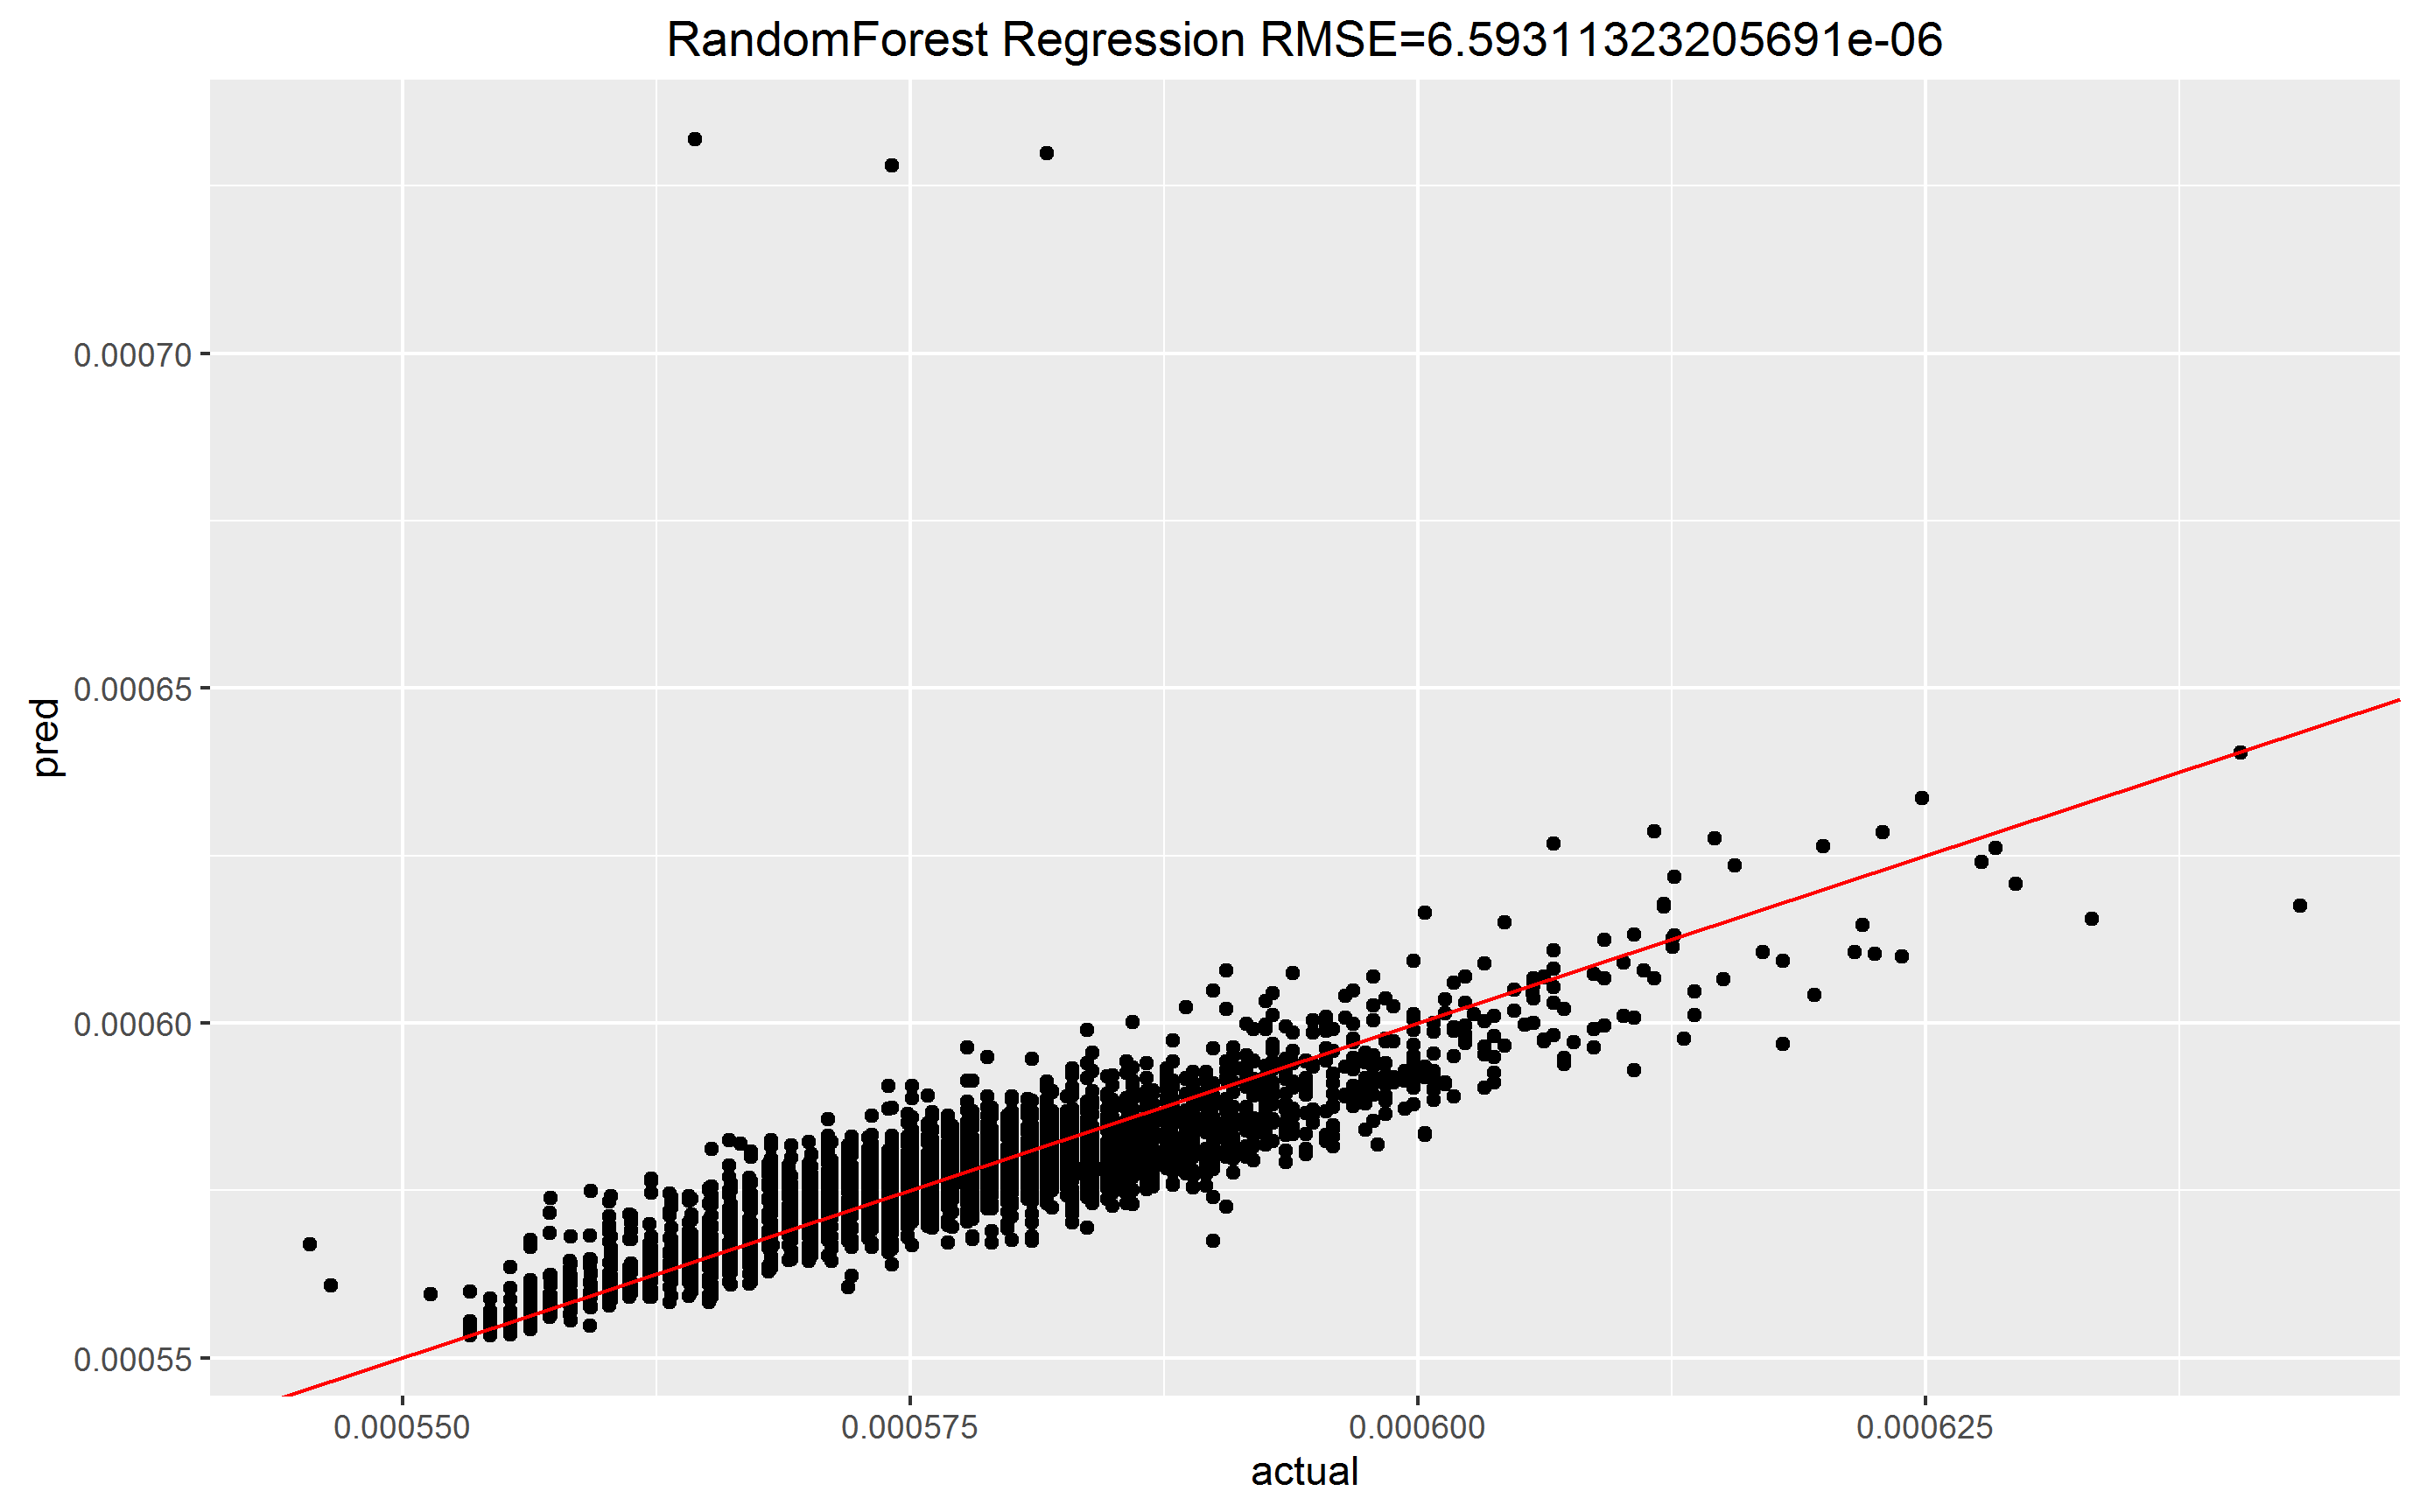
\includegraphics[width=2.25in]{Assets/Predict_24_.png}
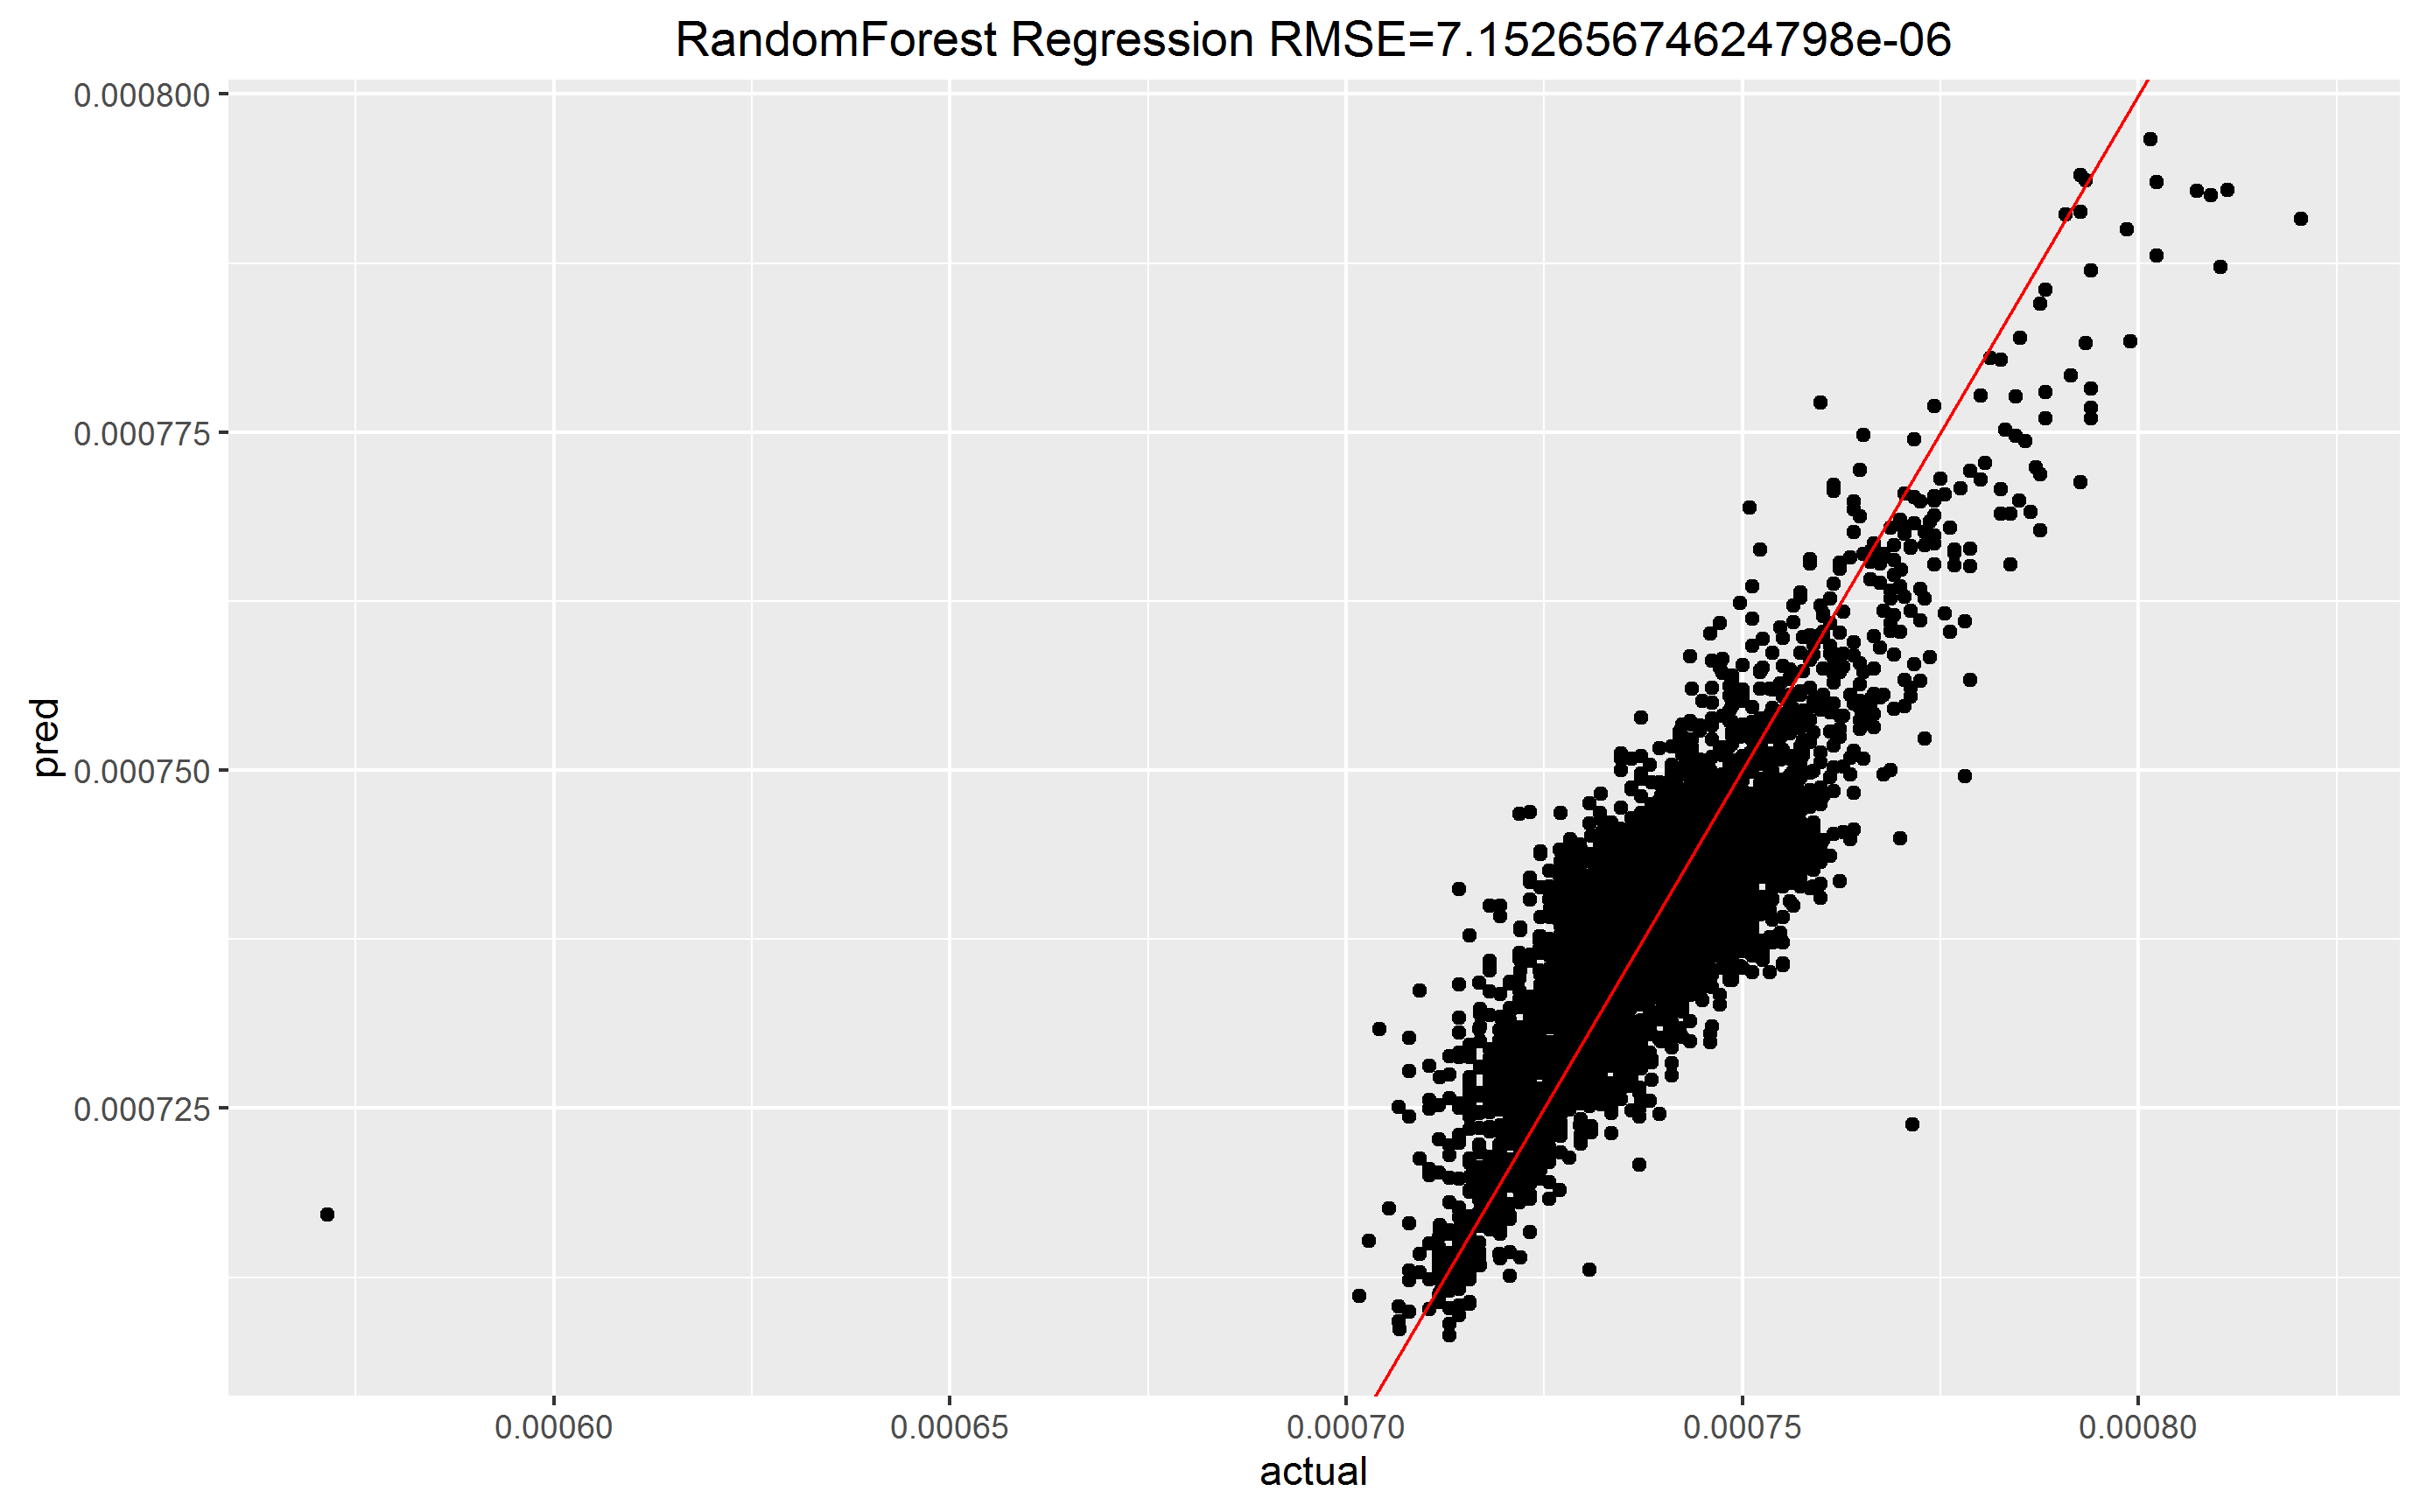
\includegraphics[width=2.25in]{Assets/Predict_5_.png}
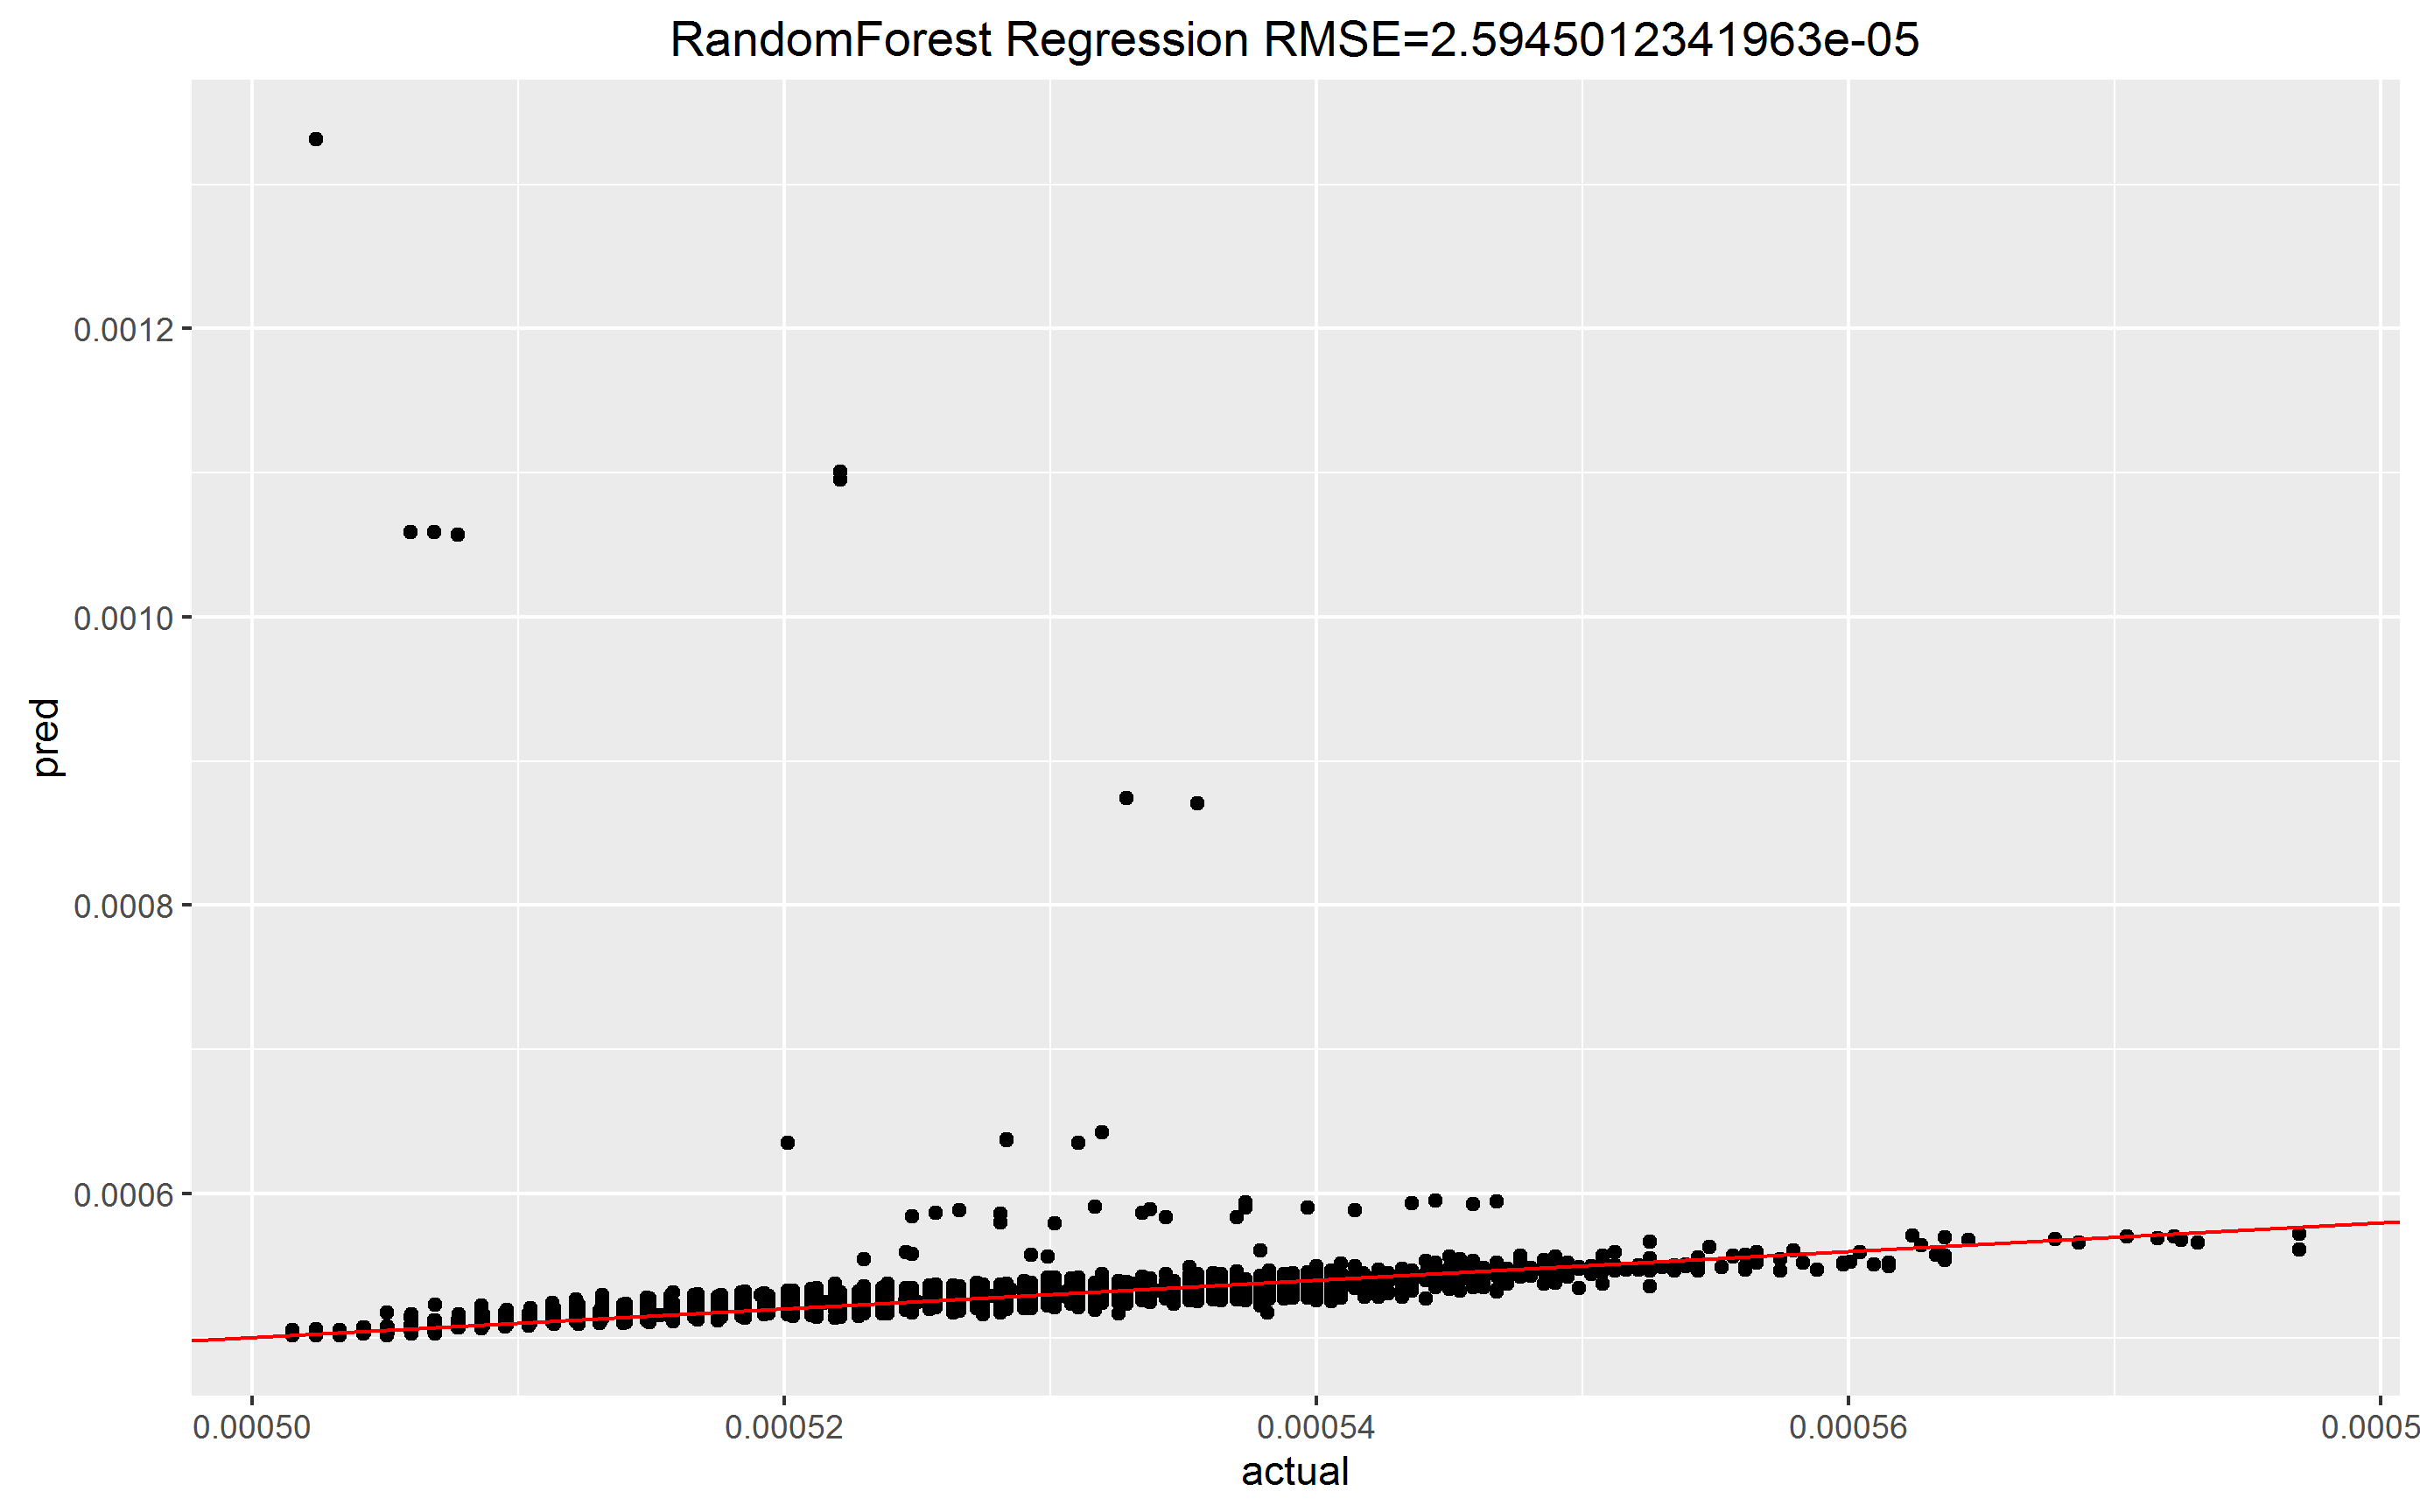
\includegraphics[width=2.25in]{Assets/Predict_29_.png}
\\Figuras 4, 5, 6. Predicción en buenos casos
\end{center}

\begin{center}
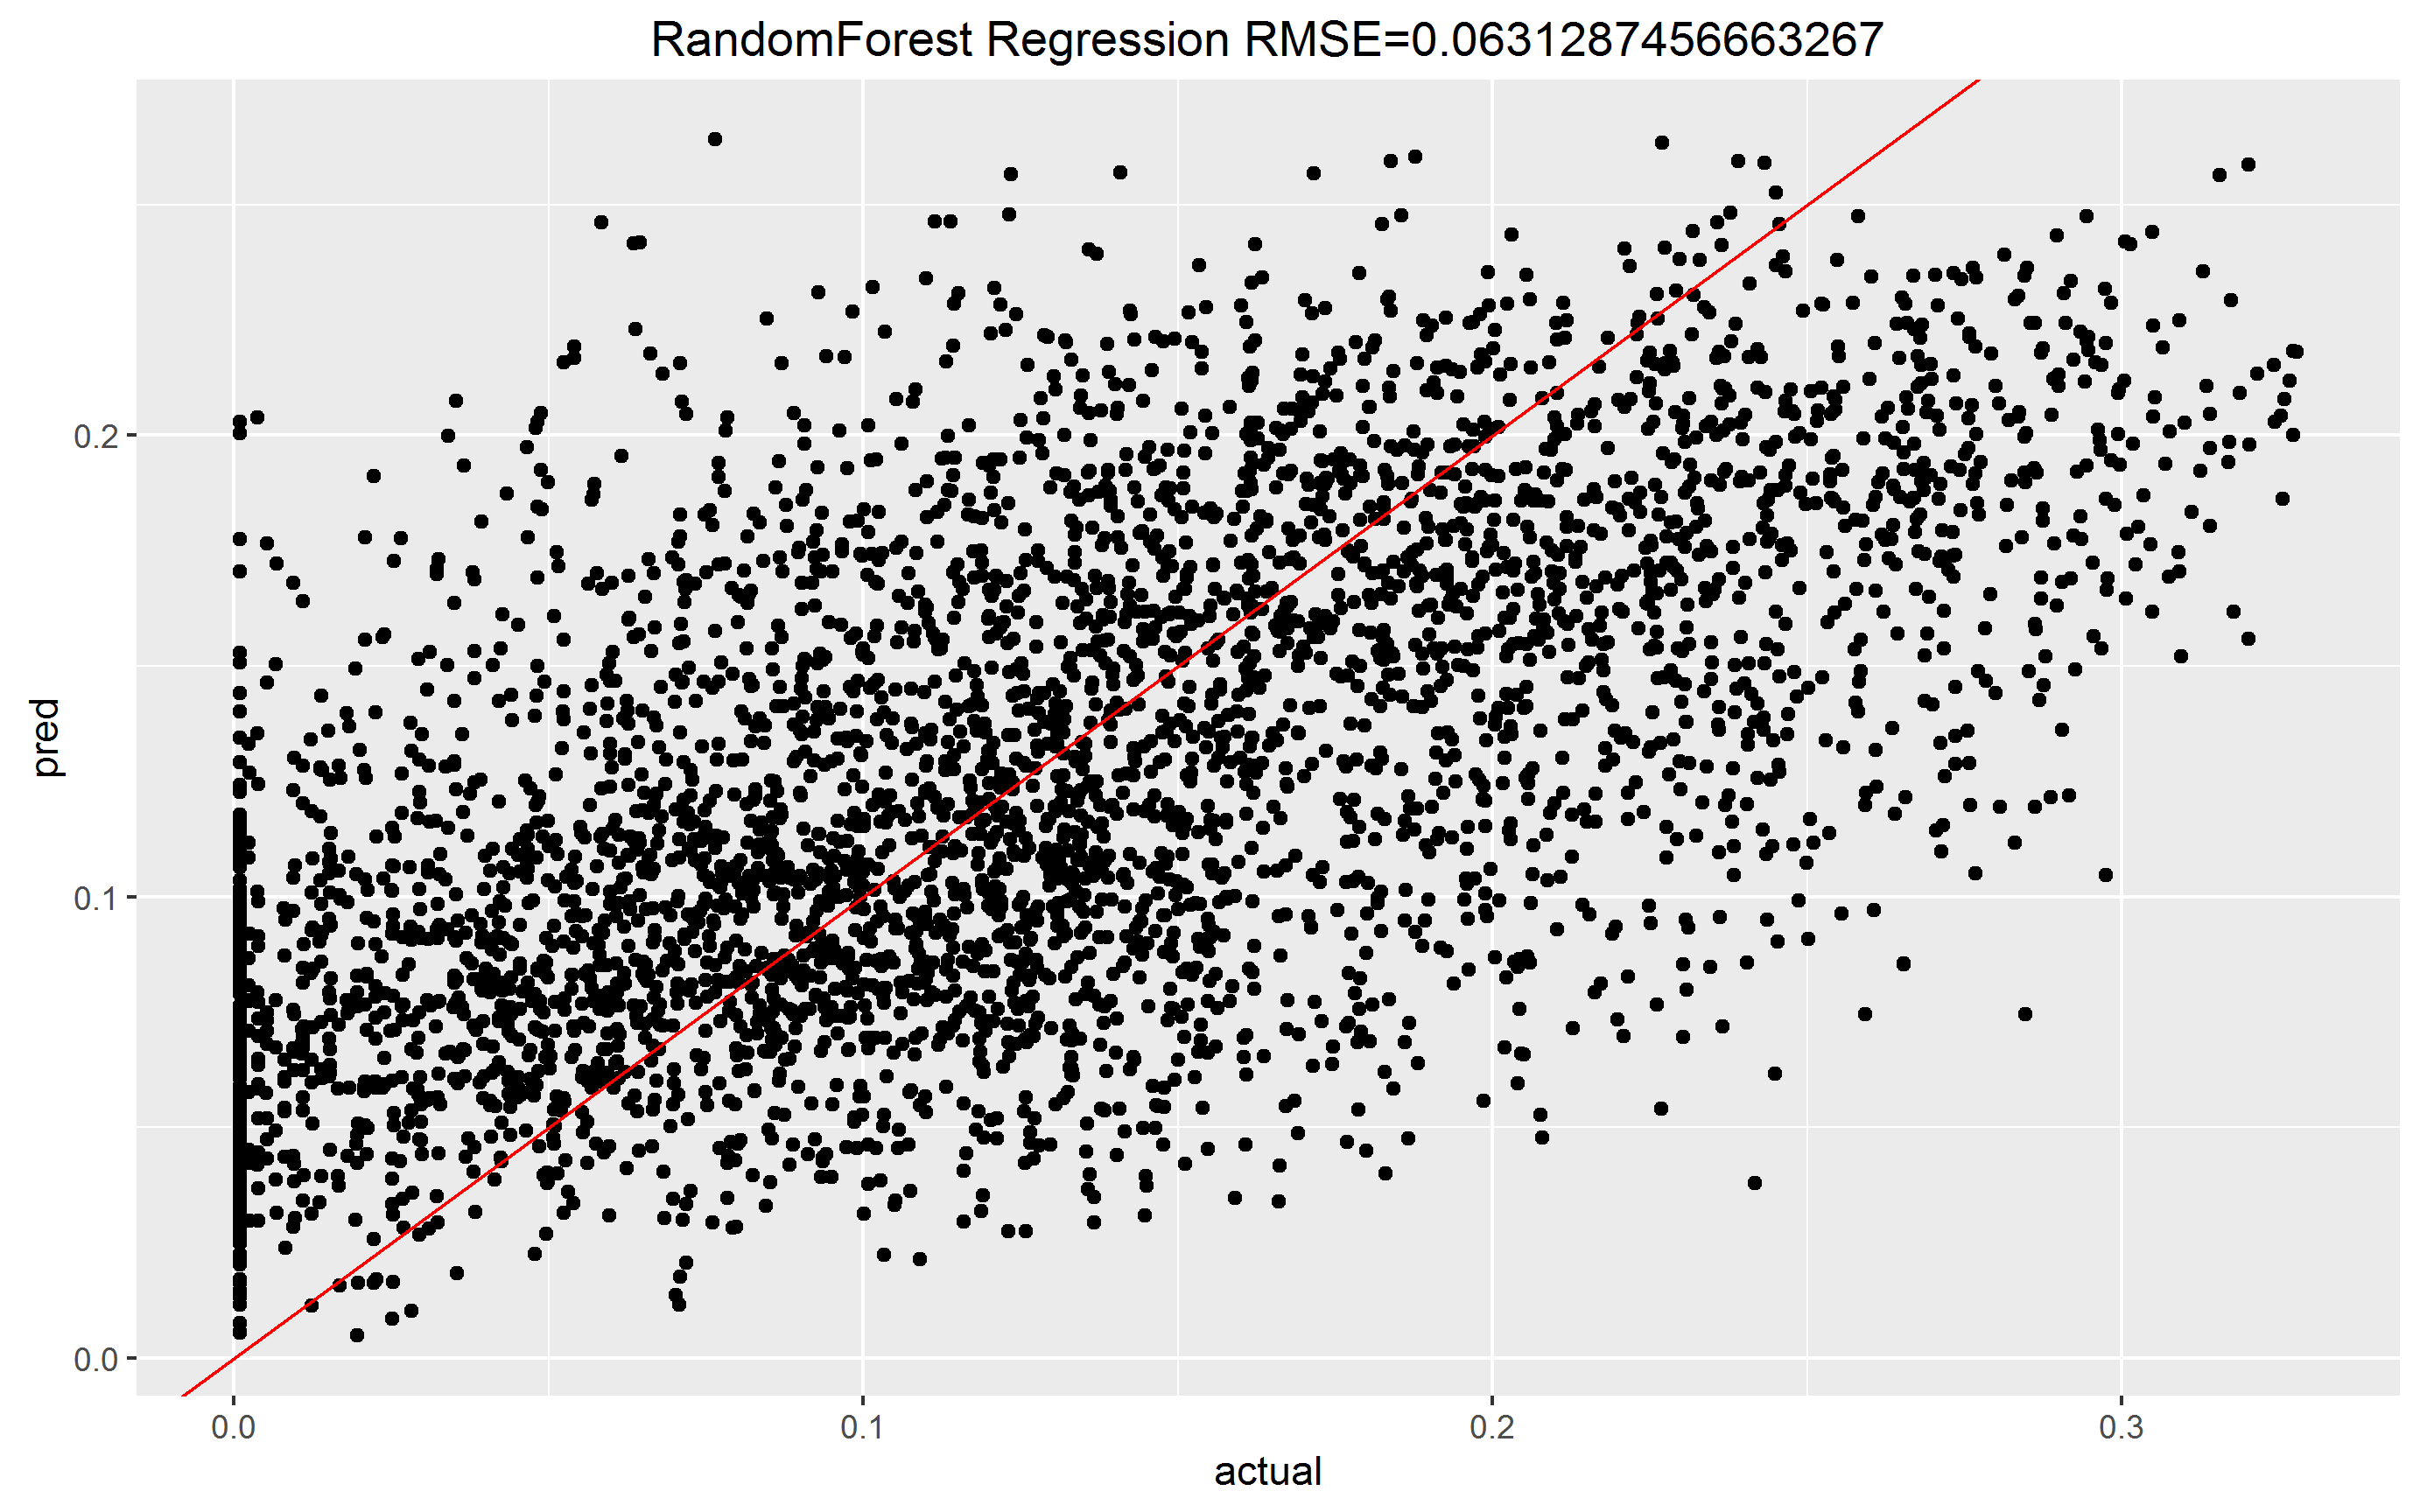
\includegraphics[width=2.25in]{Assets/Predict_19_.png}
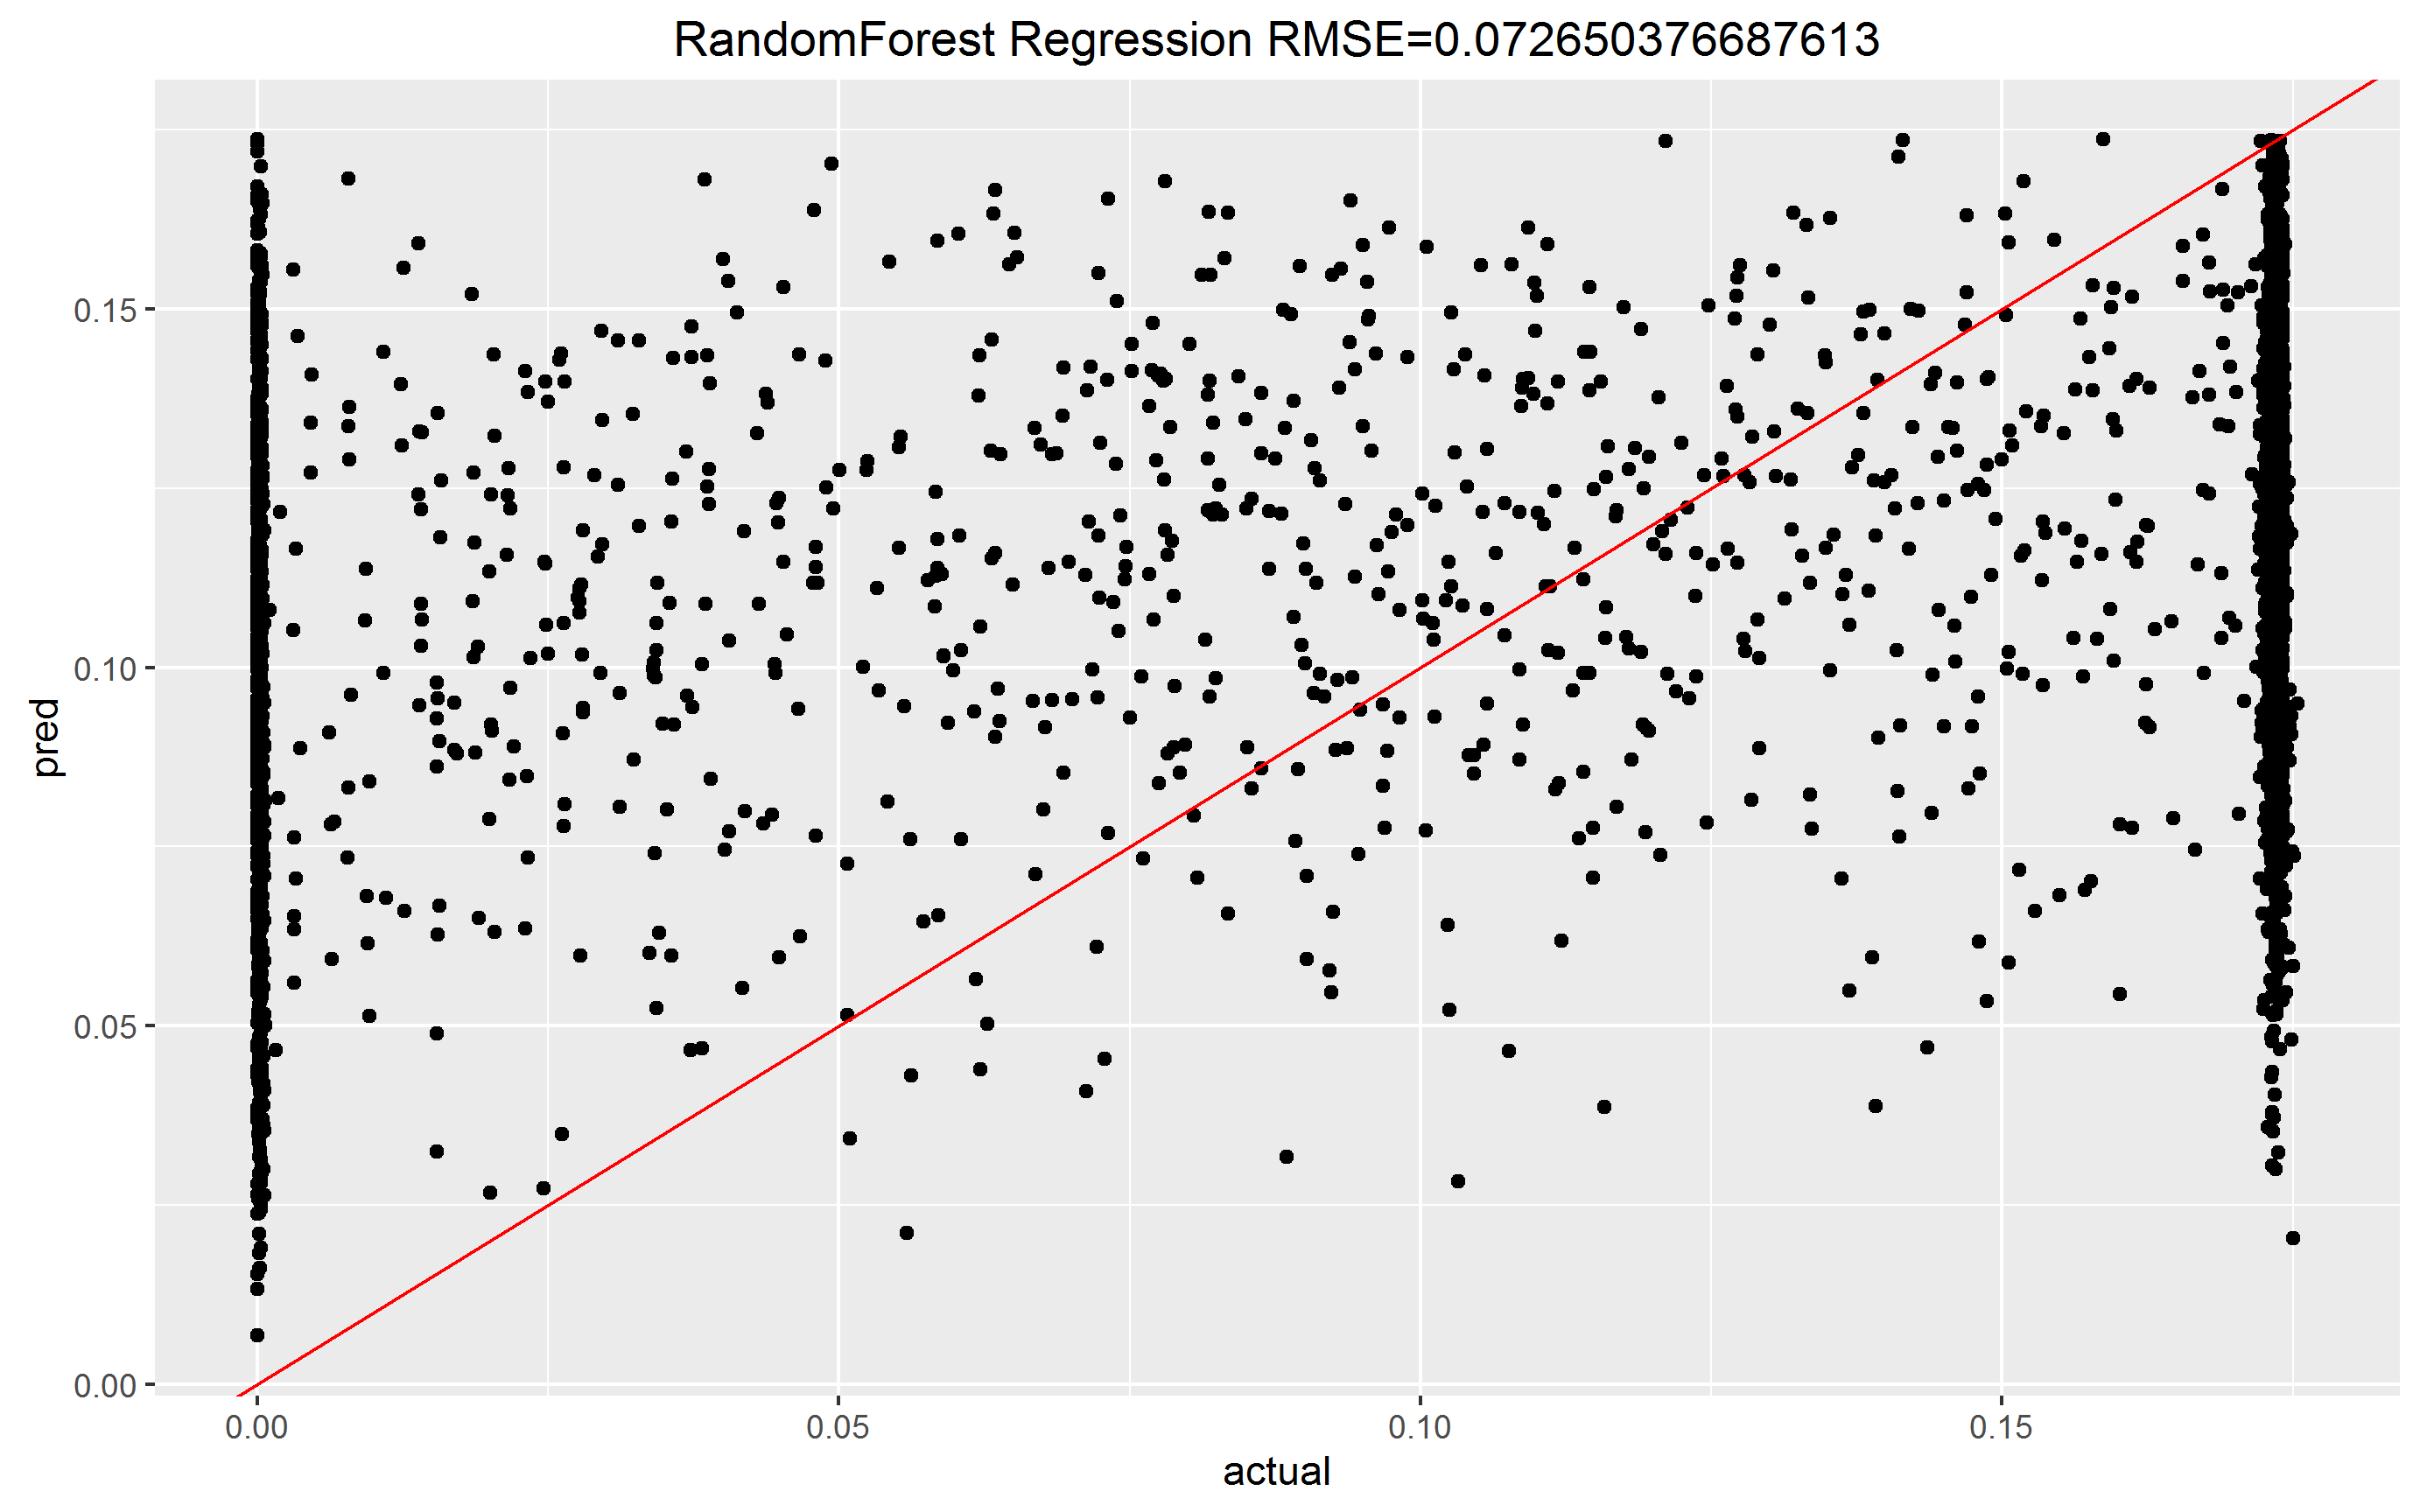
\includegraphics[width=2.25in]{Assets/Predict_23_.png}
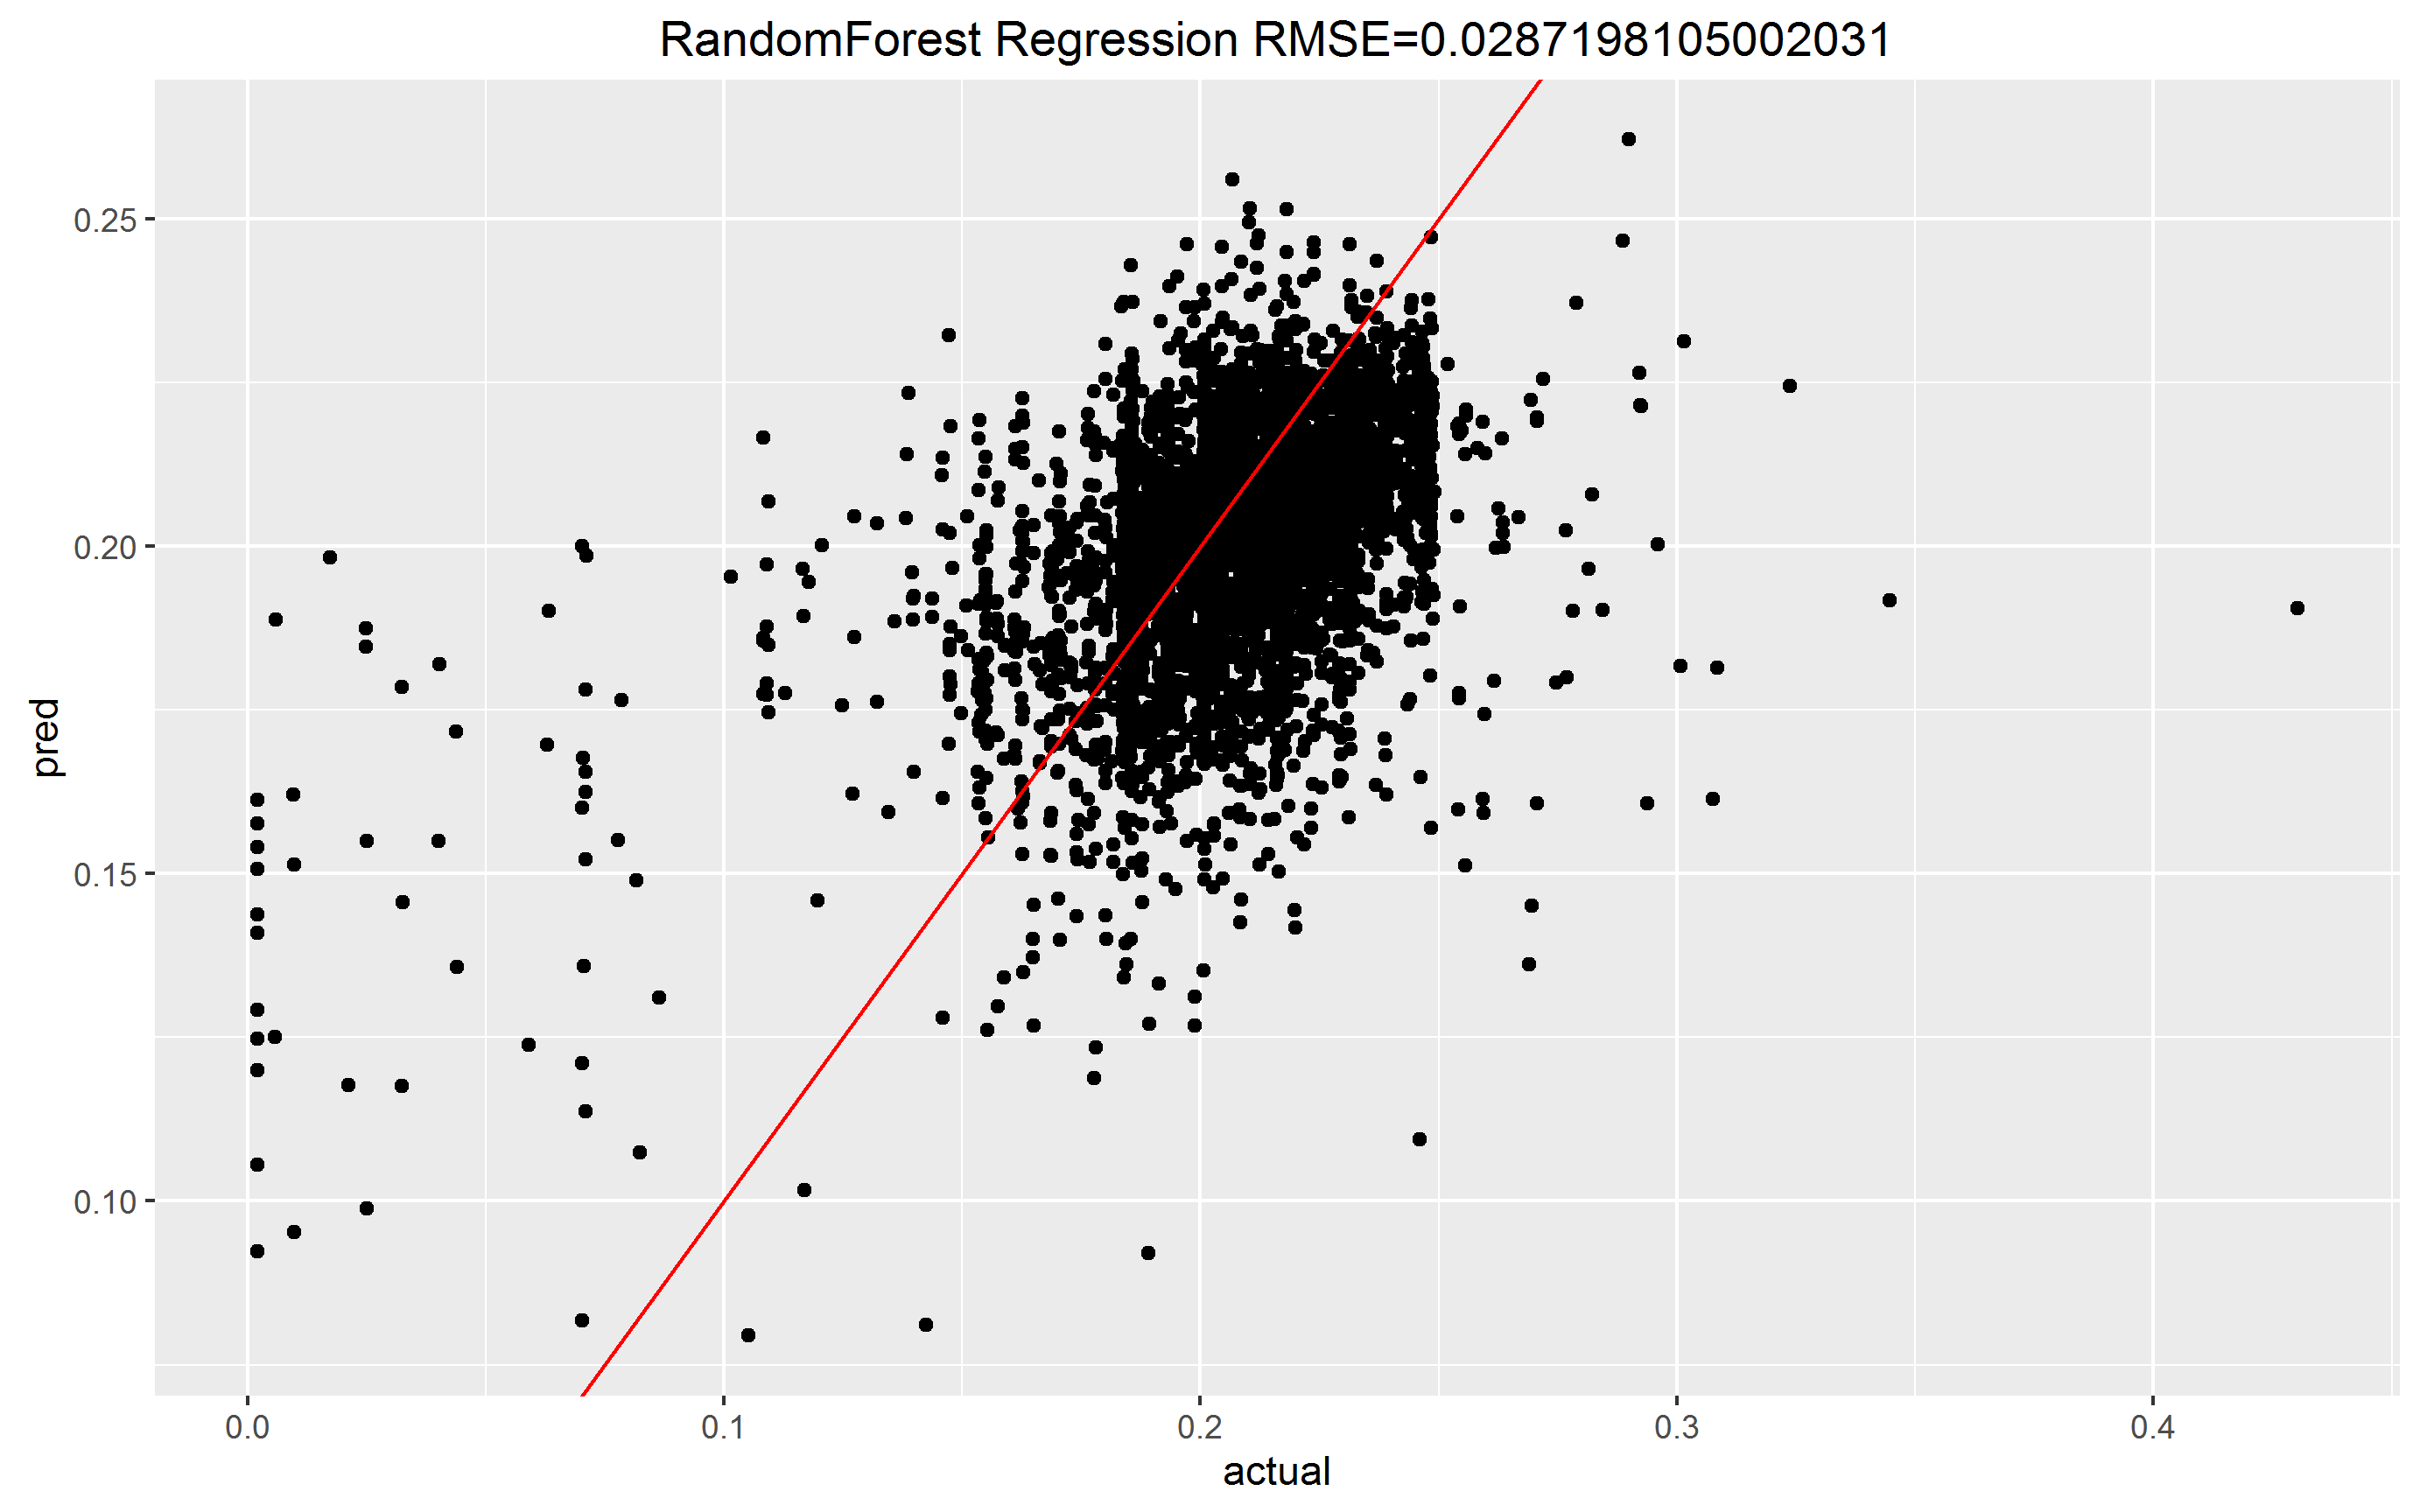
\includegraphics[width=2.25in]{Assets/Predict_9_.png}
\\Figuras 7, 8, 9. Predicción en malos casos
\end{center}

\begin{center}
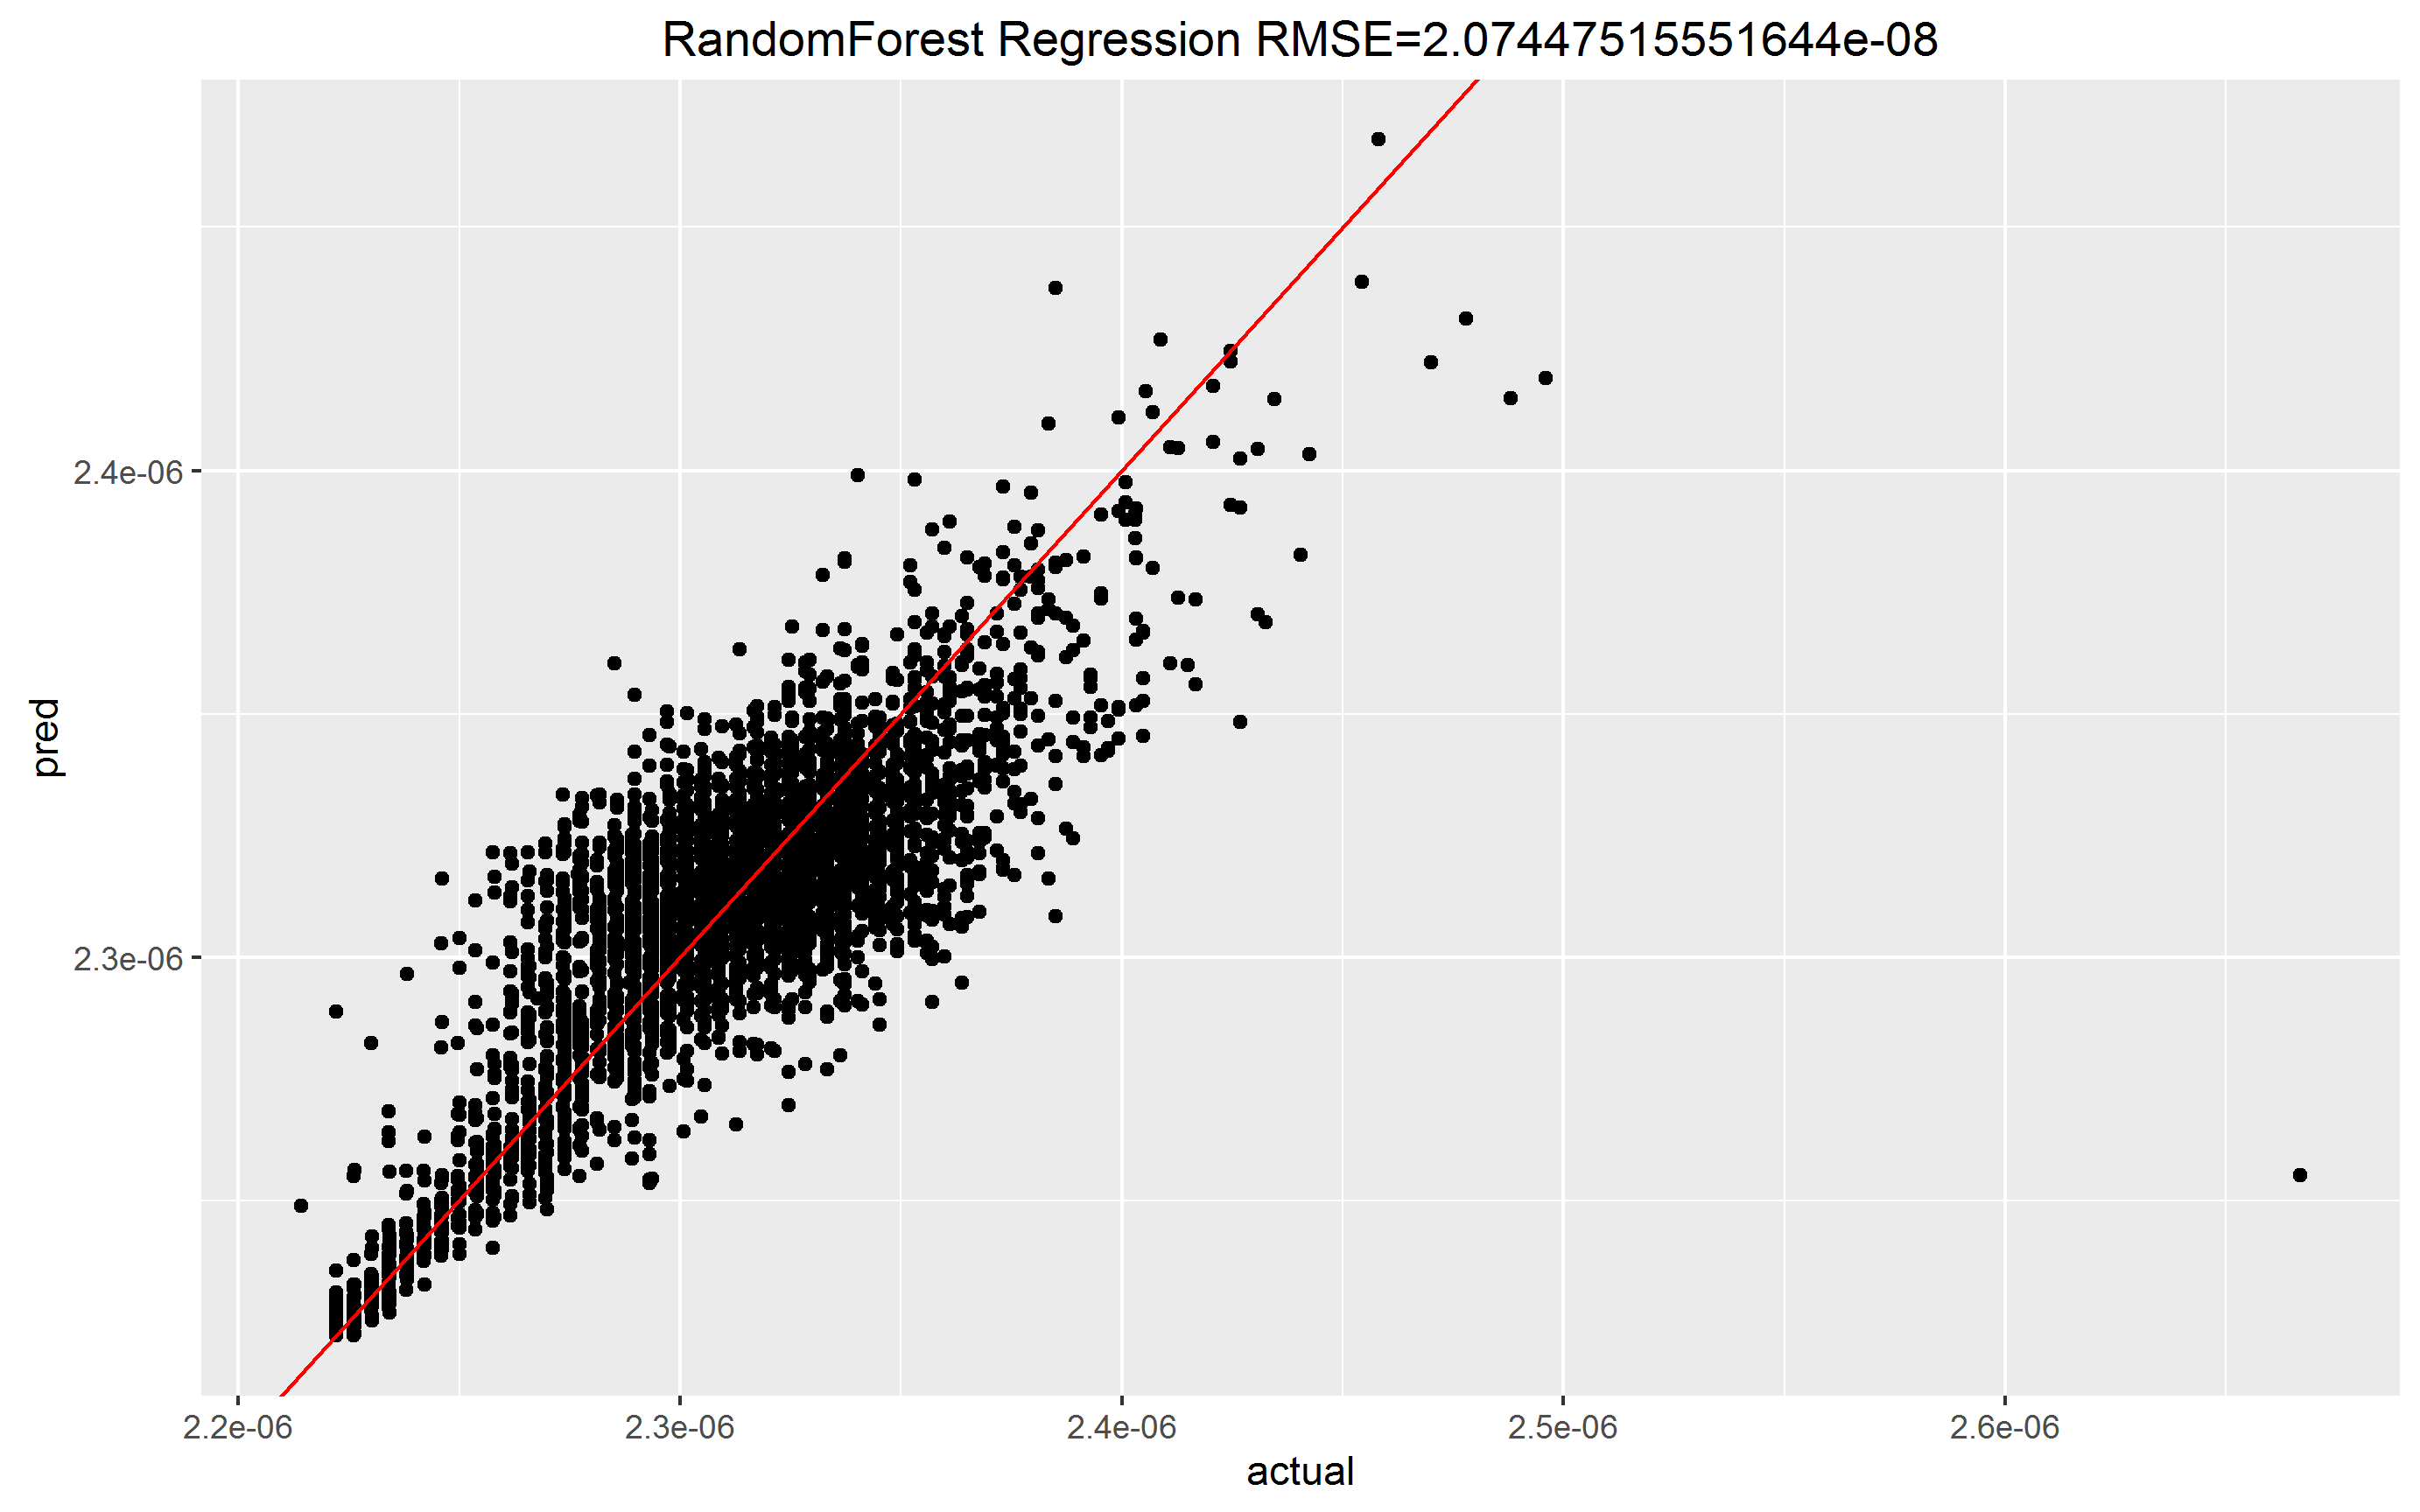
\includegraphics[width=3.4in]{Assets/Predict_17_.png}
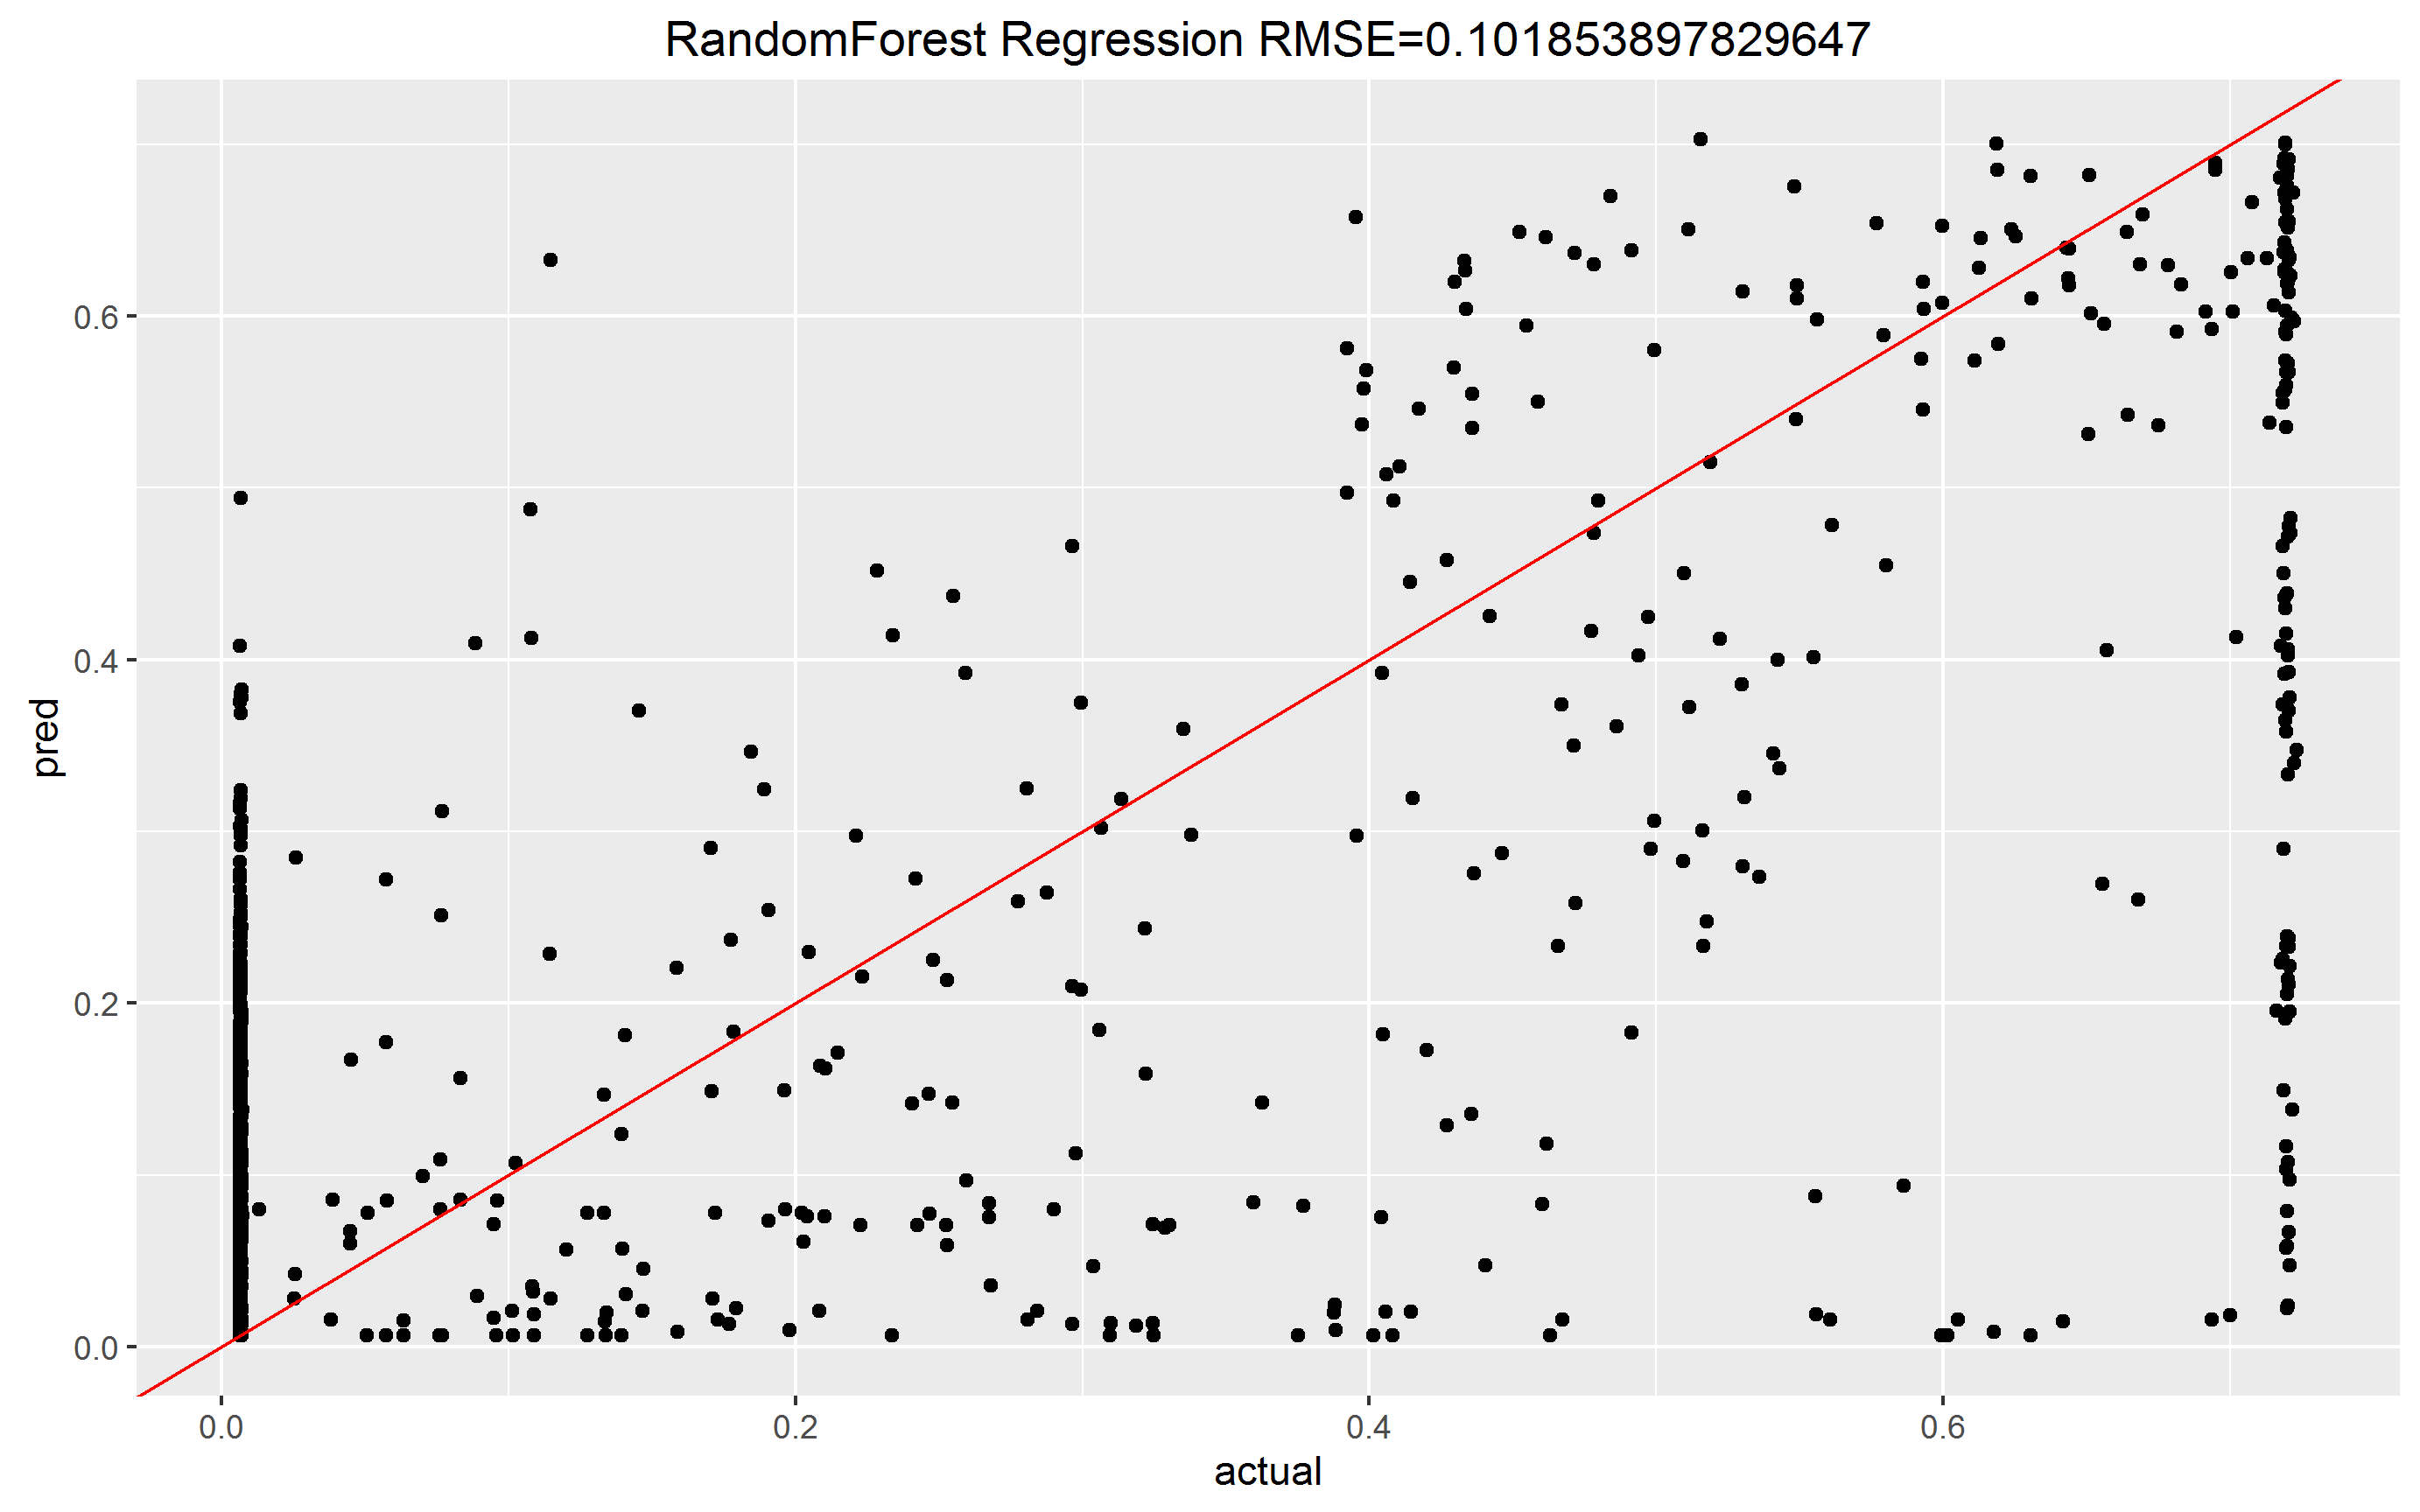
\includegraphics[width=3.4in]{Assets/Predict_32_.png}
\\Figura 10. Mejor predicción: $\epsilon=2.0744e^{-08}$
\\Figura 11. Peor predicción: $\epsilon=0.10185$
\end{center}

Como se puede apreciar, la predicción realizada tiene valores de error muy bajos. En el mejor de los casos, se pudo predecir con un $\epsilon$ de $2.0744e^{-08}$. En el peor de los casos, el error fue de $0.10185$. Al sumar el error para los 33 circuitos se pudo llegar a un error de $0.05079785$, lo cual se considera suficiente para esta experiencia.
\newline \par
Como conclusión directa de lo anterior se desprende que el consumo de potencia tiene una estrecha relación con la cantidad de energía generada, lo que es intuitivo. Esta idea afirma la hipótesis de que existe una predicción gruesa y una fina. 
\newline \par
Para poder considerar los otros sets de datos se considera realizar un pre-procesamiento adicional a los datos, como por ejemplo, encontrar la relación entre el consumo de los circuitos y la emisión de los comandos. De la misma manera, la incidencia solar tiene una dependencia sobre los eclipses solares. Este también sería una hipótesis sobre la cual avanzar.
\newline \par
Durante el (pre)procesamiento de los datos se encontraron varias dificultades, principalmente relacionadas con las capacidades computaciones. Procesar todos los datos sin agruparlos por hora conllevó tiempos extendidos, este tradeoff seguramente podría incrementar los valores de predicción, sin embargo se descarta para el desarrollo de este trabajo.
\end{document}